\documentclass[12pt,]{article}
\usepackage{lmodern}
\usepackage{amssymb,amsmath}
\usepackage{ifxetex,ifluatex}
\usepackage{fixltx2e} % provides \textsubscript
\ifnum 0\ifxetex 1\fi\ifluatex 1\fi=0 % if pdftex
  \usepackage[T1]{fontenc}
  \usepackage[utf8]{inputenc}
\else % if luatex or xelatex
  \ifxetex
    \usepackage{mathspec}
    \usepackage{xltxtra,xunicode}
  \else
    \usepackage{fontspec}
  \fi
  \defaultfontfeatures{Mapping=tex-text,Scale=MatchLowercase}
  \newcommand{\euro}{€}
    \setmainfont{Palatino}
    \setsansfont{Century Gothic}
    \setmonofont[Mapping=tex-ansi]{Consolas}
\fi
% use upquote if available, for straight quotes in verbatim environments
\IfFileExists{upquote.sty}{\usepackage{upquote}}{}
% use microtype if available
\IfFileExists{microtype.sty}{%
\usepackage{microtype}
\UseMicrotypeSet[protrusion]{basicmath} % disable protrusion for tt fonts
}{}
\ifxetex
  \usepackage[setpagesize=false, % page size defined by xetex
              unicode=false, % unicode breaks when used with xetex
              xetex]{hyperref}
\else
  \usepackage[unicode=true]{hyperref}
\fi
\hypersetup{breaklinks=true,
            bookmarks=true,
            pdfauthor={},
            pdftitle={},
            colorlinks=true,
            citecolor=blue,
            urlcolor=blue,
            linkcolor=magenta,
            pdfborder={0 0 0}}
\urlstyle{same}  % don't use monospace font for urls
\usepackage{fancyhdr}
\pagestyle{fancy}
\pagenumbering{arabic}
\lhead{\itshape }
\chead{}
\rhead{\itshape{\nouppercase{\leftmark}}}
\lfoot{v 1.15.2}
\cfoot{}
\rfoot{\thepage}
\usepackage{color}
\usepackage{fancyvrb}
\newcommand{\VerbBar}{|}
\newcommand{\VERB}{\Verb[commandchars=\\\{\}]}
\DefineVerbatimEnvironment{Highlighting}{Verbatim}{commandchars=\\\{\}, fontsize=\scriptsize}
% Add ',fontsize=\small' for more characters per line
\newenvironment{Shaded}{}{}
\newcommand{\KeywordTok}[1]{\textcolor[rgb]{0.00,0.44,0.13}{\textbf{{#1}}}}
\newcommand{\DataTypeTok}[1]{\textcolor[rgb]{0.56,0.13,0.00}{{#1}}}
\newcommand{\DecValTok}[1]{\textcolor[rgb]{0.25,0.63,0.44}{{#1}}}
\newcommand{\BaseNTok}[1]{\textcolor[rgb]{0.25,0.63,0.44}{{#1}}}
\newcommand{\FloatTok}[1]{\textcolor[rgb]{0.25,0.63,0.44}{{#1}}}
\newcommand{\ConstantTok}[1]{\textcolor[rgb]{0.53,0.00,0.00}{{#1}}}
\newcommand{\CharTok}[1]{\textcolor[rgb]{0.25,0.44,0.63}{{#1}}}
\newcommand{\SpecialCharTok}[1]{\textcolor[rgb]{0.25,0.44,0.63}{{#1}}}
\newcommand{\StringTok}[1]{\textcolor[rgb]{0.25,0.44,0.63}{{#1}}}
\newcommand{\VerbatimStringTok}[1]{\textcolor[rgb]{0.25,0.44,0.63}{{#1}}}
\newcommand{\SpecialStringTok}[1]{\textcolor[rgb]{0.73,0.40,0.53}{{#1}}}
\newcommand{\ImportTok}[1]{{#1}}
\newcommand{\CommentTok}[1]{\textcolor[rgb]{0.38,0.63,0.69}{\textit{{#1}}}}
\newcommand{\DocumentationTok}[1]{\textcolor[rgb]{0.73,0.13,0.13}{\textit{{#1}}}}
\newcommand{\AnnotationTok}[1]{\textcolor[rgb]{0.38,0.63,0.69}{\textbf{\textit{{#1}}}}}
\newcommand{\CommentVarTok}[1]{\textcolor[rgb]{0.38,0.63,0.69}{\textbf{\textit{{#1}}}}}
\newcommand{\OtherTok}[1]{\textcolor[rgb]{0.00,0.44,0.13}{{#1}}}
\newcommand{\FunctionTok}[1]{\textcolor[rgb]{0.02,0.16,0.49}{{#1}}}
\newcommand{\VariableTok}[1]{\textcolor[rgb]{0.10,0.09,0.49}{{#1}}}
\newcommand{\ControlFlowTok}[1]{\textcolor[rgb]{0.00,0.44,0.13}{\textbf{{#1}}}}
\newcommand{\OperatorTok}[1]{\textcolor[rgb]{0.40,0.40,0.40}{{#1}}}
\newcommand{\BuiltInTok}[1]{{#1}}
\newcommand{\ExtensionTok}[1]{{#1}}
\newcommand{\PreprocessorTok}[1]{\textcolor[rgb]{0.74,0.48,0.00}{{#1}}}
\newcommand{\AttributeTok}[1]{\textcolor[rgb]{0.49,0.56,0.16}{{#1}}}
\newcommand{\RegionMarkerTok}[1]{{#1}}
\newcommand{\InformationTok}[1]{\textcolor[rgb]{0.38,0.63,0.69}{\textbf{\textit{{#1}}}}}
\newcommand{\WarningTok}[1]{\textcolor[rgb]{0.38,0.63,0.69}{\textbf{\textit{{#1}}}}}
\newcommand{\AlertTok}[1]{\textcolor[rgb]{1.00,0.00,0.00}{\textbf{{#1}}}}
\newcommand{\ErrorTok}[1]{\textcolor[rgb]{1.00,0.00,0.00}{\textbf{{#1}}}}
\newcommand{\NormalTok}[1]{{#1}}
\usepackage{graphicx,grffile}
\makeatletter
\def\maxwidth{\ifdim\Gin@nat@width>\linewidth\linewidth\else\Gin@nat@width\fi}
\def\maxheight{\ifdim\Gin@nat@height>\textheight\textheight\else\Gin@nat@height\fi}
\makeatother
% Scale images if necessary, so that they will not overflow the page
% margins by default, and it is still possible to overwrite the defaults
% using explicit options in \includegraphics[width, height, ...]{}
\setkeys{Gin}{width=\maxwidth,height=\maxheight,keepaspectratio}
\setlength{\parindent}{0pt}
\setlength{\parskip}{6pt plus 2pt minus 1pt}
\setlength{\emergencystretch}{3em}  % prevent overfull lines
\providecommand{\tightlist}{%
  \setlength{\itemsep}{0pt}\setlength{\parskip}{0pt}}
\setcounter{secnumdepth}{5}

\date{}

% Redefines (sub)paragraphs to behave more like sections
\ifx\paragraph\undefined\else
\let\oldparagraph\paragraph
\renewcommand{\paragraph}[1]{\oldparagraph{#1}\mbox{}}
\fi
\ifx\subparagraph\undefined\else
\let\oldsubparagraph\subparagraph
\renewcommand{\subparagraph}[1]{\oldsubparagraph{#1}\mbox{}}
\fi

\begin{document}

{
\hypersetup{linkcolor=black}
\setcounter{tocdepth}{3}
\tableofcontents
}
\section{POMDPs}\label{pomdps}

\emph{A Julia interface for defining, solving and simulating partially
observable Markov decision processes and their fully observable
counterparts.}

\subsection{Package Features}\label{package-features}

\begin{itemize}
\tightlist
\item
  General interface that can handle problems with discrete and
  continuous state/action/observation spaces
\item
  A number of popular state-of-the-art solvers availiable to use out of
  the box
\item
  Tools that make it easy to define problems and simulate solutions
\item
  Simple integration of custom solvers into the existing interface
\end{itemize}

\subsection{Availible Packages}\label{availible-packages}

The POMDPs.jl package contains the interface used for expressing and
solving Markov decision processes (MDPs) and partially observable Markov
decision processes (POMDPs) in the Julia programming language. The
\href{https://github.com/JuliaPOMDP}{JuliaPOMDP} community maintains
these packages. The packages currently maintained by JuliaPOMDP are as
follows:

\subsubsection{MDP solvers:}\label{mdp-solvers}

\begin{itemize}
\tightlist
\item
  \href{https://github.com/JuliaPOMDP/DiscreteValueIteration.jl}{Value
  Iteration}
\item
  \href{https://github.com/JuliaPOMDP/MCTS.jl}{Monte Carlo Tree Search}
\end{itemize}

\subsubsection{POMDP solvers:}\label{pomdp-solvers}

\begin{itemize}
\tightlist
\item
  \href{https://github.com/JuliaPOMDP/QMDP.jl}{QMDP}
\item
  \href{https://github.com/JuliaPOMDP/SARSOP.jl}{SARSOP}
\item
  \href{https://github.com/JuliaPOMDP/POMCP.jl}{POMCP}
\item
  \href{https://github.com/JuliaPOMDP/DESPOT.jl}{DESPOT}
\item
  \href{https://github.com/JuliaPOMDP/MCVI.jl}{MCVI}
\item
  \href{https://github.com/JuliaPOMDP/POMDPSolve.jl}{POMDPSolve}
\end{itemize}

\subsubsection{Support Tools:}\label{support-tools}

\begin{itemize}
\tightlist
\item
  \href{https://github.com/JuliaPOMDP/POMDPToolbox.jl}{POMDPToolbox}
\item
  \href{https://github.com/JuliaPOMDP/POMDPModels.jl}{POMDPModels}
\end{itemize}

\subsubsection{Interface Extensions:}\label{interface-extensions}

\begin{itemize}
\tightlist
\item
  \href{https://github.com/JuliaPOMDP/GenerativeModels.jl}{GenerativeModels}
\item
  \href{https://github.com/JuliaPOMDP/POMDPBounds.jl}{POMDPBounds}
\end{itemize}

\subsection{Manual Outline}\label{manual-outline}

\begin{itemize}
\tightlist
\item
  \href{index.md\#POMDPs-1}{POMDPs}

  \begin{itemize}
  \tightlist
  \item
    \href{index.md\#Package-Features-1}{Package Features}
  \item
    \href{index.md\#Availible-Packages-1}{Availible Packages}
  \item
    \href{index.md\#Manual-Outline-1}{Manual Outline}
  \end{itemize}
\item
  \href{def_pomdp.md\#Defining-a-POMDP-1}{Defining a POMDP}

  \begin{itemize}
  \tightlist
  \item
    \href{def_pomdp.md\#Functional-Form-POMDP-1}{Functional Form POMDP}
  \item
    \href{def_pomdp.md\#Tabular-Form-POMDP-1}{Tabular Form POMDP}
  \item
    \href{def_pomdp.md\#Continous-POMDP-1}{Continous POMDP}
  \end{itemize}
\item
  \href{faq.md\#Frequently-Asked-Questions-(FAQ)-1}{Frequently Asked
  Questions (FAQ)}

  \begin{itemize}
  \tightlist
  \item
    \href{faq.md\#Why-am-I-getting-a-\%22No-implemnetation-for-...\%22-error?-1}{Why
    am I getting a ``No implemnetation for \ldots{}'' error?}
  \item
    \href{faq.md\#How-do-I-save-my-policies?-1}{How do I save my
    policies?}
  \item
    \href{faq.md\#Why-do-I-need-to-put-type-assertions-pomdp::POMDP-into-the-function-signature?-1}{Why
    do I need to put type assertions pomdp::POMDP into the function
    signature?}
  \item
    \href{faq.md\#Why-are-all-the-solvers-in-seperate-modules?-1}{Why
    are all the solvers in seperate modules?}
  \end{itemize}
\item
  \href{install.md\#Installation-1}{Installation}
\item
  \href{get_started.md\#Getting-Started-1}{Getting Started}
\item
  \href{api.md\#API-Documentation-1}{API Documentation}

  \begin{itemize}
  \tightlist
  \item
    \href{api.md\#Contents-1}{Contents}
  \item
    \href{api.md\#Index-1}{Index}
  \item
    \href{api.md\#Types-1}{Types}
  \item
    \href{api.md\#Model-Functions-1}{Model Functions}
  \item
    \href{api.md\#Distribution/Space-Functions-1}{Distribution/Space
    Functions}
  \item
    \href{api.md\#Belief-Functions-1}{Belief Functions}
  \item
    \href{api.md\#Policy-and-Solver-Functions-1}{Policy and Solver
    Functions}
  \item
    \href{api.md\#Simulator-1}{Simulator}
  \item
    \href{api.md\#Utility-Tools-1}{Utility Tools}
  \item
    \href{api.md\#Constants-1}{Constants}
  \end{itemize}
\item
  \href{concepts.md\#Concepts-and-Architecture-1}{Concepts and
  Architecture}

  \begin{itemize}
  \tightlist
  \item
    \href{concepts.md\#POMDPs-and-MDPs-1}{POMDPs and MDPs}
  \item
    \href{concepts.md\#Beliefs-and-Updaters-1}{Beliefs and Updaters}
  \item
    \href{concepts.md\#Solvers-and-Policies-1}{Solvers and Policies}
  \item
    \href{concepts.md\#Simulators-1}{Simulators}
  \end{itemize}
\item
  \href{def_solver.md\#Defining-a-Solver-1}{Defining a Solver}

  \begin{itemize}
  \tightlist
  \item
    \href{def_solver.md\#Background-1}{Background}
  \item
    \href{def_solver.md\#QMDP-Algorithm-1}{QMDP Algorithm}
  \item
    \href{def_solver.md\#Requirements-for-a-Solver-1}{Requirements for a
    Solver}
  \item
    \href{def_solver.md\#Defining-the-Solver-and-Policy-Types-1}{Defining
    the Solver and Policy Types}
  \item
    \href{def_solver.md\#Writing-the-Solve-Function-1}{Writing the Solve
    Function}
  \item
    \href{def_solver.md\#Creating-an-Updater-1}{Creating an Updater}
  \item
    \href{def_solver.md\#Evaluating-the-Solver-1}{Evaluating the Solver}
  \end{itemize}
\end{itemize}

\section{Installation}\label{installation}

If you have a running Julia distriubtion (Julia 0.4 or greaer), you have
everything you need to install POMDPs.jl. To install the package, simply
run the following from the Julia REPL:

\begin{Shaded}
\begin{Highlighting}[]
\NormalTok{Pkg.add(}\StringTok{"POMDPs"}\NormalTok{) }\CommentTok{# installs the POMDPs.jl package}
\end{Highlighting}
\end{Shaded}

Once you have POMDPs.jl installed, you can install any package that is
part of the JuliaPOMDP community by running:

\begin{Shaded}
\begin{Highlighting}[]
\NormalTok{using POMDPs}
\NormalTok{POMDPs.add(}\StringTok{"SARSOP"}\NormalTok{) }\CommentTok{# installs the SARSOP solver}
\end{Highlighting}
\end{Shaded}

The code above will download and install all the dependencies
automatically. All JuliaPOMDP packages have been tested on Linux and OS
X, and most have been tested on Windows.

To get a list of all the availible packages run:

\begin{Shaded}
\begin{Highlighting}[]
\NormalTok{POMDPs.available() }\CommentTok{# prints a list of all the availible packages that can be installed with POMDPs.add}
\end{Highlighting}
\end{Shaded}

Due to the modular nature of the framework, you can install only the
solvers/support tools you plan on using. However, if you want to install
all of the supported JuliaPOMDP packages you can run the following code:

\begin{Shaded}
\begin{Highlighting}[]
\NormalTok{POMDPs.add_all() }\CommentTok{# installs all the JuliaPOMDP packages (may take a few minutes)}
\end{Highlighting}
\end{Shaded}

\section{Getting Started}\label{getting-started}

Before writing our own POMDP problems or solvers, let's try out some of
the availiable solvers and problem models availible in JuliaPOMDP.

Here is a short piece of code that solves the Tiger POMDP using SARSOP,
and evaluates the results. Note that you must have the SARSOP,
POMDPModels, and POMDPToolbox modules installed.

\begin{Shaded}
\begin{Highlighting}[]
\NormalTok{using SARSOP, POMDPModels, POMDPToolbox}

\CommentTok{# initialize problem and solver}
\NormalTok{pomdp = TigerPOMDP() }\CommentTok{# from POMDPModels}
\NormalTok{solver = SARSOPSolver() }\CommentTok{# from SARSOP}

\CommentTok{# compute a policy}
\NormalTok{policy = solve(solver, pomdp)}

\CommentTok{#evaluate the policy}
\NormalTok{belief_updater = updater(policy) }\CommentTok{# the default QMPD belief updater (discrete Bayesian filter)}
\NormalTok{init_dist = initial_state_distribution(pomdp) }\CommentTok{# from POMDPModels}
\NormalTok{hist = HistoryRecorder(max_steps=}\FloatTok{100}\NormalTok{) }\CommentTok{# from POMDPToolbox}
\NormalTok{r = simulate(hist, pomdp, policy, belief_updater, init_dist) }\CommentTok{# run 100 step simulation}
\end{Highlighting}
\end{Shaded}

The first part of the code loads the desired packages and initializes
the problem and the solver. Next, we compute a POMDP policy. Lastly, we
evaluate the results.

There are a few things to mention here. First, the TigerPOMDP type
implements all the functions required by SARSOPSolver to compute a
policy. Second, each policy has a default updater (essentially a filter
used to update the belief of the POMDP). To learn more about Updaters
check out the Concepts section.

\section{Concepts and Architecture}\label{concepts-and-architecture}

POMDPs.jl aims to coordinate the development of three software
components: 1) a problem, 2) a solver, 3) an experiment. Each of these
components has a set of abstract types associated with it and a set of
functions that allow a user to define each component's behavior in a
standardized way. An outline of the architecture is shown below.

\begin{figure}[htbp]
\centering
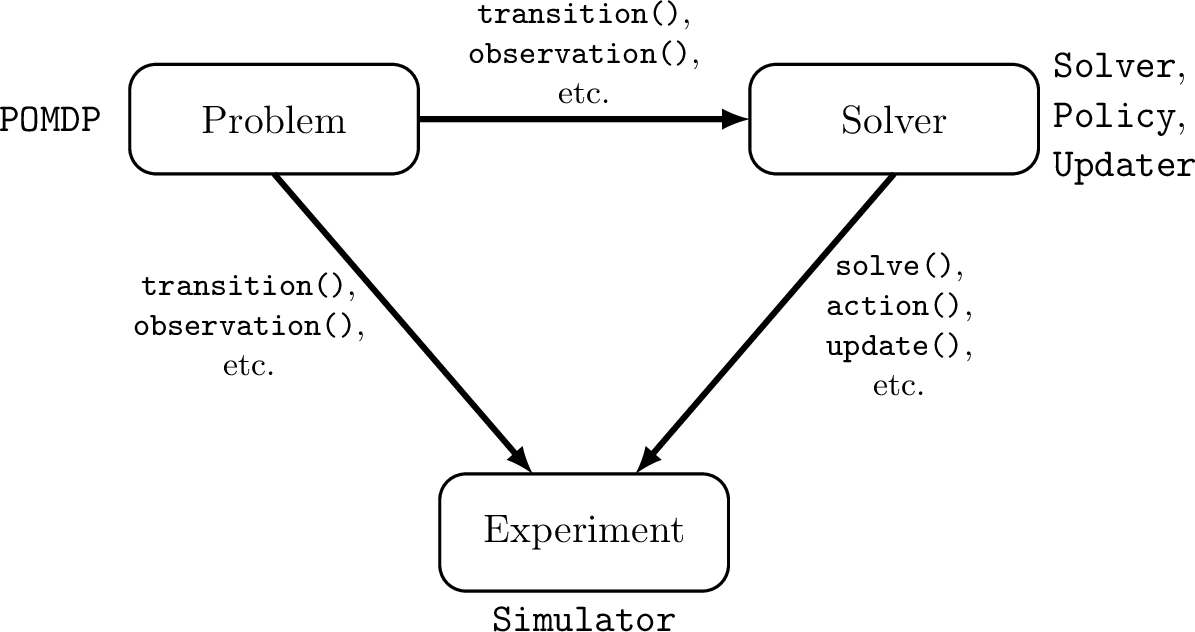
\includegraphics{figures/concepts.png}
\caption{concepts}
\end{figure}

The MDP and POMDP types are associated with the problem definition. The
Solver and Policy types are associated with the solver or
decision-making agent. Typically, the Updater type is also associated
with the solver, but a solver may sometimes be used with an updater that
was implemented separately. The Simulator type is associated with the
experiment.

\subsection{POMDPs and MDPs}\label{pomdps-and-mdps}

An MDP is a definition of a problem where the state of the problem is
fully observable. Mathematically, an MDP is a tuple (S,A,T,R), where S
is the state space, A is the action space, T is a function that defines
the probability of transitioning to each state given the state and
action at the previous time, and R is a reward function mapping every
possible transition (s,a,s') to a real reward value. For more
information see a textbook such as {[}1{]}. In POMDPs.jl an MDP is
represented by a concrete subtype of the
\href{api.md\#POMDPs.MDP}{\texttt{MDP}} abstract type and a set of
methods that define each of its components. S and A are defined by
implementing methods of the
\href{api.md\#POMDPs.states}{\texttt{states}} and
\href{api.md\#POMDPs.actions}{\texttt{actions}} functions for the
\href{api.md\#POMDPs.MDP}{\texttt{MDP}} subtype, though for some
solvers, the state space does not need to be explicitly defined. T and R
are defined by implementing methods of the
\href{api.md\#POMDPs.transition}{\texttt{transition}} and
\href{api.md\#POMDPs.reward}{\texttt{reward}} functions.

A POMDP is a problem definition where the state is only partially
observable by the decision making agent. Mathematically, a POMDP is a
tuple (S,A,T,R,O,Z) where S, A, T, and R have the same meaning as in the
MDP case, Z is the set of observations that the decision-making agent
might receive and O is a function defining the probability of receiving
each observation at a transition. In POMDPs.jl, a POMDP is represented
by a concrete subtype of the \href{api.md\#POMDPs.POMDP}{\texttt{POMDP}}
abstract type, \texttt{Z} may be defined by the
\href{api.md\#POMDPs.observations}{\texttt{observations}} function
(though an explicit definition is often not required), and \texttt{O} is
defined by implementing a method of
\href{api.md\#POMDPs.observation}{\texttt{observation}} for the POMDP
type.

POMDPs.jl also contains functions for defining optional problem behavior
such as a discount factor or a set of terminal states.

It is important to note that, in some cases, it is difficult to
explicitly represent the transition and observation distributions for a
problem but easy to generate a sampled next state or observation. In
these cases it may be significantly easier to use the
\href{https://github.com/JuliaPOMDP/GenerativeModels.jl}{\texttt{GenerativeModels.jl}}
interface extension \emph{instead of} implementing methods of
\href{api.md\#POMDPs.transition}{\texttt{transition}} and
\href{api.md\#POMDPs.observation}{\texttt{observation}}

\subsection{Beliefs and Updaters}\label{beliefs-and-updaters}

In a POMDP domain, the decision-making agent does not have complete
information about the state of the problem, so the agent can only make
choices based on its ``belief'' about the state. In the POMDP
literature, the term ``belief'' is typically defined to mean a
probability distribution over all possible states of the system.
However, in practice, the agent often makes decisions based on an
incomplete or lossy record of past observations that has a structure
much different from a probability distribution. For example, if the
agent is represented by a finite-state controller as is the case for
Monte-Carlo Value Iteration {[}2{]}, the belief is the controller state,
which is a node in a graph. Another example is an agent represented by a
recurrent neural network. In this case, the agent's belief is the state
of the network. In order to accommodate a wide variety of
decision-making approaches, in POMDPs.jl, we use the term ``belief'' to
denote the set of information that the agent makes a decision on, which
could be an exact state distribution, an action-observation history, a
set of weighted particles, or the examples mentioned before. In code,
the belief can be represented by any built-in or user defined type.

When an action is taken and a new observation is received, the belief is
updated by the belief updater. In code, a belief updater is represented
by a concrete subtype of the
\href{api.md\#POMDPs.Updater}{\texttt{Updater}} abstract type, and the
\href{api.md\#POMDPs.update}{\texttt{update}} function defines how the
belief is updated when a new observation is received.

Although the agent may use a specialized belief structure to make
decisions, the information initially given to the agent about the state
of the problem is usually most conveniently represented as a state
distribution, thus the
\href{api.md\#POMDPs.initialize_belief}{\texttt{initialize\_belief}}
function is provided to convert a state distribution to a specialized
belief structure that an updater can work with.

In many cases, the belief structure is closely related to the solution
technique, so it will be implemented by the programmer who writes the
solver. In other cases, the agent can use a variety of belief structures
to make decisions, so a domain-specific updater implemented by the
programmer that wrote the problem description may be appropriate.
Finally, some advanced generic belief updaters such as particle filters
may be implemented by a third party. The convenience function
\href{api.md\#POMDPs.updater}{\texttt{updater}} can be used to get a
suitable default updater for a policy, however many policies can work
with other updaters.

\subsection{Solvers and Policies}\label{solvers-and-policies}

Sequential decision making under uncertainty involves both online and
offline calculations. In the broad sense, the term ``solver'' as used in
the node in the figure above refers to the package of software that
performs the calculations at both of these times. However, the code is
broken up into two pieces, the solver that performs calculations offline
and the policy that performs calculations online.

In the abstract sense, a policy is a mapping from every belief that an
agent might take to an action. A policy is represented in code by a
concrete subtype of the \href{api.md\#POMDPs.Policy}{\texttt{Policy}}
abstract type. The programmer defines a method of the
\href{api.md\#POMDPs.action}{\texttt{action}} function to describe what
computations need to be done online. For an online solver such as POMCP,
all of the decision computation occurs within
\href{api.md\#POMDPs.action}{\texttt{action}} while for an offline
solver like SARSOP, there is very little computation within
\href{api.md\#POMDPs.action}{\texttt{action}}

The offline portion of the computation is carried out by the solver,
which is represented by a concrete subtype of the
\href{api.md\#POMDPs.Solver}{\texttt{Solver}} abstract type.
Computations occur within the
\href{api.md\#POMDPs.solve}{\texttt{solve}} function. For an offline
solver like SARSOP, nearly all of the decision computation occurs within
this function, but for some online solvers such as POMCP,
\href{api.md\#POMDPs.solve}{\texttt{solve}} merely embeds the problem in
the policy.

\subsection{Simulators}\label{simulators}

A simulator defines a way to run a single simulation. It is represented
by a concrete subtype of the
\href{api.md\#POMDPs.Simulator}{\texttt{Simulator}} abstract type and
the simulation is implemented in a method of the
\href{api.md\#POMDPs.simulate}{\texttt{simulate}} function.
\href{api.md\#POMDPs.simulate}{\texttt{simulate}} should return the
discounted sum of the stagewise rewards, and the simulator may or may
not keep track of the state trajectory or other statistics or display
the simulation as it is carried out.

{[}1{]} \emph{Decision Making Under Uncertainty: Theory and Application}
by Mykel J. Kochenderfer, MIT Press, 2015

{[}2{]} Bai, H., Hsu, D., \& Lee, W. S. (2014). Integrated perception
and planning in the continuous space: A POMDP approach. The
International Journal of Robotics Research, 33(9), 1288-1302

\section{Defining a POMDP}\label{defining-a-pomdp}

The expressive nature of POMDPs.jl gives problem writers the flexiblity
to write their problem in many forms. In this section we will take a
look at two ways to write a discrete problem, and a way of writing a
continuous problem.

\subsection{Functional Form POMDP}\label{functional-form-pomdp}

The first, and most straighforward way to define a POMDP problem is to
implement the model functions that you may need. For example, all POMDPs
will need \texttt{transition}, \texttt{reward}, and \texttt{observation}
functions. In this example we'll start with the simple Tiger POMDP
problem. We want to use the SARSOP solver to compute a policy. To use a
solver from JuliaPOMDP, a problem writer must define a set of functions
required by the solver. To see what functions are required by SARSOP,
check out its documentation \protect\hyperlink{href}{here}.

Let's first define the Tiger POMDP type.

\begin{Shaded}
\begin{Highlighting}[]
\NormalTok{using POMDPs }\CommentTok{# load the interface}
\CommentTok{# parametarized inheritance POMDP\{state, action, observation\}}
\KeywordTok{type} \NormalTok{TigerPOMDP <: POMDP\{}\DataTypeTok{Bool}\NormalTok{, }\DataTypeTok{Int64}\NormalTok{, }\DataTypeTok{Bool}\NormalTok{\} }
    \NormalTok{r_listen::}\DataTypeTok{Float64} \CommentTok{# reward for listening (negative)}
    \NormalTok{r_findtiger::}\DataTypeTok{Float64} \CommentTok{# reward for finding the tiger (negative)}
    \NormalTok{r_escapetiger::}\DataTypeTok{Float64} \CommentTok{# reward for escaping}
    \NormalTok{p_listen_correctly::}\DataTypeTok{Float64} \CommentTok{# probbility that we hear the tiger correctly}
    \NormalTok{discount_factor::}\DataTypeTok{Float64} \CommentTok{# discount factor}
\KeywordTok{end}
\NormalTok{TigerPOMDP() = TigerPOMDP(-}\FloatTok{1.0}\NormalTok{, -}\FloatTok{100.0}\NormalTok{, }\FloatTok{10.0}\NormalTok{, }\FloatTok{0.85}\NormalTok{, }\FloatTok{0.95}\NormalTok{) }\CommentTok{# default contructor}
\end{Highlighting}
\end{Shaded}

Notice that the \texttt{TigerPOMDP} is inheriting from the abstract
\texttt{POMDP} type that comes from POMDPs.jl. The abstract
\texttt{POMDP} is parametarized by a \texttt{Bool}, \texttt{Int64},
\texttt{Bool} combination with the syntax
\texttt{TigerPOMDP\ \textless{}:\ POMDP\{Bool,\ Int64,\ Bool\}}. The
parametarization defines how we choose to represent the state, actions,
and observations in our problem. In the \texttt{TigerPOMDP} we use a
boolean to represent our states and observations (because there are two
of each) and an integer to represent our actions (because there are 3).
If you wanted to create a custom concrete type to represent your states,
actions, or observations you could do that as well. Let's say we made a
type to represent our states called \texttt{AwesomeTigerState}. That
type could contain integers, floats, arrays, or other complex data
structures (depending on what's convenient). We would then parametrize
the Tiger POMDP in the following way:
\texttt{type\ TigerPOMDP\ \textless{}:\ POMDP\{AwesomeTigerState,\ Int64,\ Bool\}}.

Now, let's consider another important component of POMDPs, probability
distributions. In the POMDPs.jl interface, we think in terms of
distribution types. We want to be able to sample from these
distriubtions and compute their probability masses or densities. In the
Tiger POMDP, our distriubtions are over binary variables (boolean state
or observation), so we can implement a simple version of a Bernoulli
distribution.

\begin{Shaded}
\begin{Highlighting}[]
\KeywordTok{type} \NormalTok{TigerDistribution <: AbstractDistribution }\CommentTok{# inherits from a POMDPs.jl abstract type}
    \NormalTok{p::}\DataTypeTok{Float64} \CommentTok{# probability of 1}
    \NormalTok{it::}\DataTypeTok{Vector}\NormalTok{\{}\DataTypeTok{Bool}\NormalTok{\} }\CommentTok{# pre-allocate the domain of the distriubtion}
\KeywordTok{end}
\NormalTok{TigerDistribution() = TigerDistribution(}\FloatTok{0.5}\NormalTok{, [true, false]) }\CommentTok{# default constructo}

\CommentTok{# convenience function used by discrete solvers (iterator over the discrete distriubtion)}
\NormalTok{iterator(d::TigerDistribution) = d.it }
\end{Highlighting}
\end{Shaded}

Let's implement the pdf and rand function that returns the probability
mass and samples from the distribution.

\begin{Shaded}
\begin{Highlighting}[]
\CommentTok{# returns the probability mass }
\KeywordTok{function} \NormalTok{pdf(d::TigerDistribution, so::}\DataTypeTok{Bool}\NormalTok{)}
    \NormalTok{so ? (}\KeywordTok{return} \NormalTok{d.p) : (}\KeywordTok{return} \FloatTok{1.0}\NormalTok{-d.p)}
\KeywordTok{end}

\CommentTok{# samples the dsitribution}
\NormalTok{rand(rng::AbstractRNG, d::TigerDistribution, s::}\DataTypeTok{Bool}\NormalTok{) = rand(rng) <= d.p}
\end{Highlighting}
\end{Shaded}

We also want some convenience functions for initializing the
distriubtions.

\begin{Shaded}
\begin{Highlighting}[]
\NormalTok{create_transition_distribution(::TigerPOMDP) = TigerDistribution()}
\NormalTok{create_observation_distribution(::TigerPOMDP) = TigerDistribution()}
\end{Highlighting}
\end{Shaded}

Let's define our transition, observation, and reward functions.

\begin{Shaded}
\begin{Highlighting}[]
\KeywordTok{function} \NormalTok{transition(pomdp::TigerPOMDP, s::}\DataTypeTok{Bool}\NormalTok{,
a::}\DataTypeTok{Int64}\NormalTok{,}
                   \NormalTok{ d::TigerDistribution=create_transition_distribution(pomdp))}
    \CommentTok{# Resets the problem after opening door; does nothing after listening        }
    \KeywordTok{if} \NormalTok{a == }\FloatTok{1} \NormalTok{|| a == }\FloatTok{2}
        \NormalTok{d.p = }\FloatTok{0.5}
    \KeywordTok{elseif} \NormalTok{s}
        \NormalTok{d.p = }\FloatTok{1.0}
    \KeywordTok{else}
        \NormalTok{d.p = }\FloatTok{0.0}
    \KeywordTok{end}
    \NormalTok{d}
\KeywordTok{end}

\KeywordTok{function} \NormalTok{observation(pomdp::TigerPOMDP, s::}\DataTypeTok{Bool}\NormalTok{,
a::}\DataTypeTok{Int64}\NormalTok{,}
                    \NormalTok{ d::TigerDistribution=create_observation_distribution(pomdp))}
    \CommentTok{# correct observation wiht prob pc        }
    \NormalTok{pc = pomdp.p_listen_correctly}
    \KeywordTok{if} \NormalTok{a == }\FloatTok{0}
        \NormalTok{s ? (d.p = pc) : (d.p = }\FloatTok{1.0}\NormalTok{-pc)}
    \KeywordTok{else}
        \NormalTok{d.p = }\FloatTok{0.5}
    \KeywordTok{end}
    \NormalTok{d}
\KeywordTok{end}
\CommentTok{# convenience function}
\KeywordTok{function} \NormalTok{observation(pomdp::TigerPOMDP, s::}\DataTypeTok{Bool}\NormalTok{,
a::}\DataTypeTok{Int64}\NormalTok{, sp::}\DataTypeTok{Bool}\NormalTok{, }
                     \NormalTok{d::TigerDistribution=create_observation_distribution(pomdp))}
    \KeywordTok{return} \NormalTok{observation(pomdp, s, a, d)}
\KeywordTok{end}

\KeywordTok{function} \NormalTok{reward(pomdp::TigerPOMDP, s::}\DataTypeTok{Bool}\NormalTok{, a::}\DataTypeTok{Int64}\NormalTok{)}
    \CommentTok{# rewarded for escaping, penalized for listening and getting caught}
    \NormalTok{r = }\FloatTok{0.0}
    \NormalTok{a == }\FloatTok{0} \NormalTok{? (r+=pomdp.r_listen) : (nothing)}
    \KeywordTok{if} \NormalTok{a == }\FloatTok{1}
        \NormalTok{s ? (r += pomdp.r_findtiger) : (r += pomdp.r_escapetiger)}
    \KeywordTok{end}
    \KeywordTok{if} \NormalTok{a == }\FloatTok{2}
        \NormalTok{s ? (r += pomdp.r_escapetiger) : (r += pomdp.r_findtiger)}
    \KeywordTok{end}
    \KeywordTok{return} \NormalTok{r}
\KeywordTok{end}
\CommentTok{# convenience function}
\NormalTok{reward(pomdp::TigerPOMDP, s::}\DataTypeTok{Bool}\NormalTok{, a::}\DataTypeTok{Int64}\NormalTok{, sp::}\DataTypeTok{Bool}\NormalTok{) = reward(pomdp, s, a)}
\end{Highlighting}
\end{Shaded}

The last important component of a POMDP are the spaces. There is a
special \texttt{AbstractSpace} type in POMDPs.jl which all spaces
inherit from. We define the state, action, and observation spaces below
as well as functions for intializing them and sampling from them.

\begin{Shaded}
\begin{Highlighting}[]
\CommentTok{# STATE SPACE}
\KeywordTok{type} \NormalTok{TigerStateSpace <: AbstractSpace}
    \NormalTok{states::}\DataTypeTok{Vector}\NormalTok{\{}\DataTypeTok{Bool}\NormalTok{\} }\CommentTok{# states are boolean}
\KeywordTok{end}
\CommentTok{# initialize the state space}
\NormalTok{states(::TigerPOMDP) = TigerStateSpace([true, false])}
\CommentTok{# for iterating over discrete spaces}
\NormalTok{iterator(space::TigerStateSpace) = space.states}
\NormalTok{dimensions(::TigerStateSpace) = }\FloatTok{1}
\CommentTok{# sample from the state sapce}
\NormalTok{rand(rng::AbstractRNG, space::TigerStateSpace, s::}\DataTypeTok{Bool}\NormalTok{) =}
                                \NormalTok{rand(rng) > }\FloatTok{0.5} \NormalTok{? (}\KeywordTok{return} \NormalTok{true) : (}\KeywordTok{return} \NormalTok{false)}

\CommentTok{# ACTION SPACE}
\KeywordTok{type} \NormalTok{TigerActionSpace <: AbstractSpace}
    \NormalTok{actions::}\DataTypeTok{Vector}\NormalTok{\{}\DataTypeTok{Int64}\NormalTok{\} }\CommentTok{# three possible actions}
\KeywordTok{end}
\CommentTok{# initialize the action space}
\NormalTok{actions(::TigerPOMDP) = TigerActionSpace([}\FloatTok{0}\NormalTok{,}\FloatTok{1}\NormalTok{,}\FloatTok{2}\NormalTok{])}
\CommentTok{# iterate of the action space}
\NormalTok{iterator(space::TigerActionSpace) = space.actions}
\NormalTok{dimensions(::TigerActionSpace) = }\FloatTok{1}
\CommentTok{# sample from the aciton space}
\NormalTok{rand(rng::AbstractRNG, space::TigerActionSpace, a::}\DataTypeTok{Int64}\NormalTok{) = rand(rng, }\FloatTok{0}\NormalTok{:}\FloatTok{2}\NormalTok{)}

\CommentTok{# OBSERVATION SPACE}
\KeywordTok{type} \NormalTok{TigerObservationSpace <: AbstractSpace}
    \NormalTok{obs::}\DataTypeTok{Vector}\NormalTok{\{}\DataTypeTok{Bool}\NormalTok{\}}
\KeywordTok{end}
\CommentTok{# initialize}
\NormalTok{observations(::TigerPOMDP) = TigerObservationSpace([true, false])}
\CommentTok{# iterate over obs space}
\NormalTok{iterator(space::TigerObservationSpace) = space.obs}
\NormalTok{dimensions(::TigerObservationSpace) = }\FloatTok{1}
\CommentTok{# sample from the obs sapce}
\NormalTok{rand(rng::AbstractRNG, space::TigerObservationSpace, s::}\DataTypeTok{Bool}\NormalTok{) =}
                                    \NormalTok{rand(rng) > }\FloatTok{0.5} \NormalTok{? (}\KeywordTok{return} \NormalTok{true) : (}\KeywordTok{return} \NormalTok{false)}
\end{Highlighting}
\end{Shaded}

The last important component of a POMDP is the initial distribution over
the state space. In POMDPs.jl we make a strong distinction between this
distribution and a belief. In most literature these two concepts are
considered the same. However, in most general terms, a belief is
something that is mapped to an action using a POMDP policy. If the
policy is represented as something other than alpha-vectors (a policy
graph, tree, or a reccurent neural netowrk to give a few examples), it
may not make sense to think of a belief as a probability distribution
over the state space. Thus, in POMDPs.jl we abstract the concept of a
belief beyond a probability distribution (of course it can be a
probability distriubtion if it makes sense).

In order to reconcile this difference, each policy has a function called
\texttt{initialize\_belief} which takes in an initial state distirubtion
(this is a probability distribution over the state space) and a policy,
and converts the distribution into what we call a belief in POMDPs.jl -
a representation of a POMDP that is mapped to an action using the
policy.

Let's define the initial state distribution function for our POMDP.

\begin{Shaded}
\begin{Highlighting}[]
\NormalTok{initial_state_distribution(pomdp::TigerPOMDP) = TigerDistribution(}\FloatTok{0.5}\NormalTok{, [true, false])}
\end{Highlighting}
\end{Shaded}

Now that've defined all the main components, we need to wrap up our
model by creating some convenience functions below.

\begin{Shaded}
\begin{Highlighting}[]
\CommentTok{# initialization functions}
\NormalTok{create_state(::TigerPOMDP) = zero(}\DataTypeTok{Bool}\NormalTok{)}
\NormalTok{create_observation(::TigerPOMDP) = zero(}\DataTypeTok{Bool}\NormalTok{)}
\NormalTok{create_action(::TigerPOMDP) = zero(}\DataTypeTok{Int64}\NormalTok{)}

\CommentTok{# for discrete problems}
\NormalTok{n_states(::TigerPOMDP) = }\FloatTok{2}
\NormalTok{n_actions(::TigerPOMDP) = }\FloatTok{3}
\NormalTok{n_observations(::TigerPOMDP) = }\FloatTok{2}

\CommentTok{# for indexing discrete states}
\NormalTok{state_index(::TigerPOMDP, s::}\DataTypeTok{Bool}\NormalTok{) = }\DataTypeTok{Int64}\NormalTok{(s) + }\FloatTok{1}

\NormalTok{discount(pomdp::TigerPOMDP) = pomdp.discount_factor}
\end{Highlighting}
\end{Shaded}

Now that we've defined all these functions, we can use one of the
JuliaPOMDP solvers to compute and evaluate a policy.

\begin{Shaded}
\begin{Highlighting}[]
\NormalTok{using QMDP, POMDPToolbox}

\NormalTok{pomdp = TigerPOMDP()}
\NormalTok{solver = QMDPSolver()}
\NormalTok{policy = solve(solver, pomdp)}

\NormalTok{init_dist = initial_state_distribution(pomdp)}
\NormalTok{hist = HistoryRecorder(max_steps=}\FloatTok{100}\NormalTok{) }\CommentTok{# from POMDPToolbox}
\NormalTok{r = simulate(hist, pomdp, policy, belief_updater, init_dist) }\CommentTok{# run 100 step simulation}
\end{Highlighting}
\end{Shaded}

Please note that you do not need to define all the functions for most
solvers. If you want to use an individual solver, you usually need only
a subset of what's above.

\subsection{Tabular Form POMDP}\label{tabular-form-pomdp}

Another way to define discrete POMDP problems is by writing them in
tabular form. Specifically, if you can write the transition and
observation probabilities as well as the rewards in matrix form, you can
use the \texttt{DiscreteMDP} or \texttt{DiscretePOMDP} types form
\texttt{POMDPModels} which automatically implements all the functions
you'll need for you. Let's do this with the Tiger POMDP.

\begin{Shaded}
\begin{Highlighting}[]
\NormalTok{using POMDPModels}

\CommentTok{# write out the matrix forms}

\CommentTok{# REWARDS}
\NormalTok{R = [-}\FloatTok{1}\NormalTok{. -}\FloatTok{100} \FloatTok{10}\NormalTok{; -}\FloatTok{1} \FloatTok{10} \NormalTok{-}\FloatTok{100}\NormalTok{] }\CommentTok{# |S|x|A| state-action pair rewards}

\CommentTok{# TRANSITIONS}
\NormalTok{T = zeros(}\FloatTok{2}\NormalTok{,}\FloatTok{3}\NormalTok{,}\FloatTok{2}\NormalTok{) }\CommentTok{# |S|x|A|x|S|, T[s', a, s] = p(s'|a,s)}
\NormalTok{T[:,:,}\FloatTok{1}\NormalTok{] = [}\FloatTok{1}\NormalTok{. }\FloatTok{0.5} \FloatTok{0.5}\NormalTok{; }\FloatTok{0} \FloatTok{0.5} \FloatTok{0.5}\NormalTok{]}
\NormalTok{T[:,:,}\FloatTok{2}\NormalTok{] = [}\FloatTok{0}\NormalTok{. }\FloatTok{0.5} \FloatTok{0.5}\NormalTok{; }\FloatTok{1} \FloatTok{0.5} \FloatTok{0.5}\NormalTok{]}

\CommentTok{# OBSERVATIONS}
\NormalTok{O = zeros(}\FloatTok{2}\NormalTok{,}\FloatTok{3}\NormalTok{,}\FloatTok{2}\NormalTok{) }\CommentTok{# |O|x|A|x|S|, O[o, a, s] = p(o|a,s)}
\NormalTok{O[:,:,}\FloatTok{1}\NormalTok{] = [}\FloatTok{0.85} \FloatTok{0.5} \FloatTok{0.5}\NormalTok{; }\FloatTok{0.15} \FloatTok{0.5} \FloatTok{0.5}\NormalTok{]}
\NormalTok{O[:,:,}\FloatTok{2}\NormalTok{] = [}\FloatTok{0.15} \FloatTok{0.5} \FloatTok{0.5}\NormalTok{; }\FloatTok{0.85} \FloatTok{0.5} \FloatTok{0.5}\NormalTok{]}

\NormalTok{discount = }\FloatTok{0.95}
\NormalTok{pomdp = DiscretePOMDP(T, R, O, discount)}

\CommentTok{# solve the POMDP the same way}
\NormalTok{solver = SARSOPSolver()}
\NormalTok{policy = solve(solver, pomdp)}
\end{Highlighting}
\end{Shaded}

It is usually fairly simple to define smaller problems in the tabular
form. However, for larger problems it can be tedious and the functional
form may be preffered. You can usually use any supported POMDP solver to
sovle these types of problems (the performance of the policy may vary
however - SARSOP will usually outperform QMDP).

\subsection{Continous POMDP}\label{continous-pomdp}

Within the POMDPs.jl interface, we can also define problems with
continuous spaces. There are a few solvers that can handle these types
of problems, namely, MCVI and POMCP (with some tunning). Light-Dark
problem here. What should we say about bounds?

\section{Defining a Solver}\label{defining-a-solver}

In this section, we will walk through an implementation of the
\href{http://www-anw.cs.umass.edu/~barto/courses/cs687/Cassandra-etal-POMDP.pdf}{QMDP}
algorithm. QMDP is the fully observable approximation of a POMDP policy,
and relies on the Q-values to determine actions.

\subsection{Background}\label{background}

Let's say we are working with a POMDP defined by the tuple
\((\mathcal{S}, \mathcal{A}, \mathcal{Z}, T, R, O, \gamma)\), where
\(\mathcal{S}\), \(\mathcal{A}\), \(\mathcal{Z}\) are the of discrete
state, action, and observation spaces respectively. The QMDP algorithm
assumes that the POMDP its solving is discrete. In our model
\(T : \mathcal{S} \times \mathcal{A} \times \mathcal{S} \rightarrow [0, 1]\)
is the transition function,
\(R: \mathcal{S} \times \mathcal{A} \rightarrow \mathbb{R}\) is the
reward function, and
\(O: \mathcal{Z} \times \mathcal{A} \times \mathcal{S} \rightarrow [0,1]\)
is the observation function. In a POMDP, our goal is to compute a policy
\(\pi\) that maps beliefs to actions \(\pi: b \rightarrow a\). For QMDP,
a belief can be represented by a discrete probability distribution over
the state space (although there may be other ways to define a belief in
general and POMDPs.jl allows this flexibility).

Before thinking about how we can compute a policy, lets first think of
how we can write the optimal value function for a POMDP. Recall that in
an MDP, the optimal value function simply represents the maximum
expected utility from a given state. The idea is similar in a POMDP, but
now we can think of the optimal value function with respect to a belief,
and not just a single state. Since our belief is a probability
distribution over the states, we can write the value function as
follows:

\(U^{*}(b) = \max_{a} \sum_{s} b(s)R(s,a)\)

If we let \(\alpha_{a}\) represent \(R(:,a)\) as a vector, and \(b\)
represent our distribution over state (i.e.~belief), then we can write
above as

\(U^{*}(b) = \max_{a} \alpha_{a}^{T}b\)

The \(\alpha_{a}\) in the equation above is what's often called an alpha
vector. These alpha vectors can be though of as compact representations
of a POMDP policy. Just as in an MDP, we often want to compute the
Q-matrix, in a POMDP, we want to compute these alpha vectors. Note that
an alpha vectors can be though of as a part of a piecewise linear and
convex approximation to a POMDP value function (which is itself convex).
Also note that using \(R(:,a)\) as an approximation for an alpha vectors
will often give you a very poor approximation. So now that we know that
we must compute these alpha vectors, how do we do it?

\subsection{QMDP Algorithm}\label{qmdp-algorithm}

One of the simplest algorithms for computing these alpha vectors is
known as QMDP. It uses the Q-matrix \(Q(s,a)\) obtained by solving the
MDP associated with the POMDP, and setting each alpha vector equal to
the columns of that matrix \(\alpha_{a} = Q(:, s)\). If you are familiar
with the value iteration algorithm for MDPs, the procedure for finding
these alpha vectors is identical. Let's first initialize the alpha
vectors \(\alpha_{a}^{0} = 0\) for all \(s\), and then iterate

\(\alpha_{a}^{k+1}(s) = R(s,a) + \gamma \sum_{s'} T(s'|s,a) \max_{a'} \alpha_{a'}^{k}(s')\)

After enough iterations, the alpha vectors converge to the QMDP
approximation.

Remember that QMDP is just an approximation method, and does not
guarantee that the alpha vectors you obtain actually represent your
POMDP value function. Specifically, QMDP has trouble in problems with
information gathering actions (because we completely ignored the
observation function when computing our policy). However, QMDP works
very well in problems where a particular choice of action has little
impact on the reduction in state uncertainty.

\subsection{Requirements for a Solver}\label{requirements-for-a-solver}

Before getting into the implementation details, let's first go through
what a POMDP solver must be able to do and support. We need three custom
types that inherit from abstract types in POMDPs.jl. These type are
Solver, Policy, and Updater. It is usaully useful to have a custom type
that represents the belief used by your policy as well.

The requirements are as follows:

\begin{Shaded}
\begin{Highlighting}[]
\CommentTok{# types }
\NormalTok{QMDPSolver}
\NormalTok{QMDPPolicy}
\NormalTok{DiscreteUpdater }\CommentTok{# already implemented for us in POMDPToolbox}
\NormalTok{DiscreteBelief }\CommentTok{# already implemented for us in POMDPToolbox}
\CommentTok{# methods}
\NormalTok{create_policy(solver::QMDPSolver, pomdp::POMDP) }\CommentTok{# initalizes a QMDP policy}
\NormalTok{create_belief(up::DiscreteUpdater) }\CommentTok{# initializes a QMDP belief}
\NormalTok{updater(p::QMDPPolicy) }\CommentTok{# initializes a QMDP belief udpater}
\CommentTok{# returns a QMDP belief}
\NormalTok{initialize_belief(bu::QMDPUpdater, initial_state_dist::AbstractDistribution) }
\NormalTok{solve(solver::QMDPSolver, pomdp::POMDP) }\CommentTok{# solver the POMDP and returns a policy}
\CommentTok{# returns an updated belied (already implemented)}
\NormalTok{update\{A,O\}(bu::DiscreteUpdater, belief_old::DiscreteBelief, action::A, obs::O) }
\NormalTok{action(policy::QMDPPolicy, b::DiscreteBelief) }\CommentTok{# returns a QMDP action}
\end{Highlighting}
\end{Shaded}

You can find the implementations of these types and mehtods below.

\subsection{Defining the Solver and Policy
Types}\label{defining-the-solver-and-policy-types}

Let's first define the Solver type. The QMDP solver type should contain
all the information needed to compute a policy (other than the problem
itself). This information can be though of as the hyperparameters of the
solver. In QMDP, we only need two hyper-parameters. We may want to set
the maximum number of iterations that the algorithm runs for, and a
tolerance value (also known as the Bellman residual). Both of these
quantities define terminating criteria for the algorithm. The algorithm
stops either when the maximum number of iterations has been reached or
when the infinity norm of the diference in utility values between two
iterations goes below the tolerance value. The type definition has the
form:

\begin{Shaded}
\begin{Highlighting}[]
\NormalTok{using POMDPs }\CommentTok{# first load the POMDPs module}
\KeywordTok{type} \NormalTok{QMDPSolver <: Solver}
    \NormalTok{max_iterations::}\DataTypeTok{Int64} \CommentTok{# max number of iterations QMDP runs for}
    \NormalTok{tolerance::}\DataTypeTok{Float64} \CommentTok{# Bellman residual: terminates when max||Ut-Ut-1|| < tolerance}
\KeywordTok{end}
\CommentTok{# default constructor}
\NormalTok{QMDPSolver(;max_iterations::}\DataTypeTok{Int64}\NormalTok{=}\FloatTok{100}\NormalTok{,
tolerance::}\DataTypeTok{Float64}\NormalTok{=}\FloatTok{1e-3}\NormalTok{) =}
                                    \NormalTok{QMDPSolver(max_iterations, tolerance)}
\end{Highlighting}
\end{Shaded}

Note that the QMDPSolver inherits from the abstract Solver type that's
part of POMDPs.jl.

Now, let's define a policy type. In general, the policy should contain
all the information needed to map a belief to an action. As mentioned
earlier, we need alpha vectors to be part of our policy. We can
represent the alpha vectors using a matrix of size
\(\mathcal{S} \times \mathcal{A}\). Recall that in POMDPs.jl, the
actions can be represented in a number of ways (Int64, concrete types,
etc), so we need a way to map these actions to integers so we can index
into our alpha matrix. The type looks like:

\begin{Shaded}
\begin{Highlighting}[]
\KeywordTok{type} \NormalTok{QMDPPolicy <: Policy}
    \NormalTok{alphas::}\DataTypeTok{Matrix}\NormalTok{\{}\DataTypeTok{Float64}\NormalTok{\} }\CommentTok{# matrix of alpha vectors |S|x|A|}
    \NormalTok{action_map::}\DataTypeTok{Vector}\NormalTok{\{}\DataTypeTok{Any}\NormalTok{\} }\CommentTok{# maps indices to actions}
    \NormalTok{pomdp::POMDP            }\CommentTok{# models for convenience}
\KeywordTok{end}
\CommentTok{# default constructor}
\KeywordTok{function} \NormalTok{QMDPPolicy(pomdp::POMDP)}
    \NormalTok{ns = n_states(pomdp)}
    \NormalTok{na = n_actions(pomdp)}
    \NormalTok{alphas = zeros(ns, na)}
    \NormalTok{am = }\DataTypeTok{Any}\NormalTok{[]}
    \NormalTok{space = actions(pomdp)}
    \KeywordTok{for} \NormalTok{a }\KeywordTok{in} \NormalTok{iterator(space)}
        \NormalTok{push!(am, a)}
    \KeywordTok{end}
    \KeywordTok{return} \NormalTok{QMDPPolicy(alphas, am, pomdp)}
\KeywordTok{end}
\CommentTok{# initalization function (required by POMDPs.jl)}
\NormalTok{POMDPs.create_policy(solver::QMDPSolver, pomdp::POMDP) = QMDPPolicy(pomdp)}
\end{Highlighting}
\end{Shaded}

Now that we have our solver and policy types, we can write the solve
function to compute the policy.

\subsection{Writing the Solve
Function}\label{writing-the-solve-function}

The solve function takes in a solver, a pomdp, and an optional policy
argument. Let's compute those alpha vectors!

\begin{Shaded}
\begin{Highlighting}[]
\KeywordTok{function} \NormalTok{POMDPs.solve(solver::QMDPSolver, pomdp::POMDP, policy::QMDPPolicy=create_policy(solver, pomdp))}

    \CommentTok{# get solver parameters}
    \NormalTok{max_iterations = solver.max_iterations}
    \NormalTok{tolerance = solver.tolerance}
    \NormalTok{discount_factor = discount(pomdp)}

    \CommentTok{# intialize the alpha-vectors}
    \NormalTok{alphas = policy.alphas}

    \CommentTok{# pre-allocate the transtion distirbution and the interpolants}
    \CommentTok{# we use the POMDPs.jl function for initializing a transition distribution    }
    \NormalTok{dist = create_transition_distribution(pomdp)}

    \CommentTok{# initalize space}
    \NormalTok{sspace = states(pomdp)  }\CommentTok{# returns a discrete state space object of the pomdp}
    \NormalTok{aspace = actions(pomdp) }\CommentTok{# returns a discrete action space object}

    \CommentTok{# main loop}
    \KeywordTok{for} \NormalTok{i = }\FloatTok{1}\NormalTok{:max_iterations}
        \NormalTok{residual = }\FloatTok{0.0}
        \CommentTok{# state loop}
        \CommentTok{# the iterator function returns an iterable object (array, iterator, etc) over a discrete space}
        \KeywordTok{for} \NormalTok{(istate, s) }\KeywordTok{in} \NormalTok{enumerate(iterator(sspace))}
            \NormalTok{old_alpha = maximum(alphas[istate,:]) }\CommentTok{# for residual }
            \NormalTok{max_alpha = -Inf}
            \CommentTok{# action loop}
            \CommentTok{# alpha(s) = R(s,a) + discount_factor * sum(T(s'|s,a)max(alpha(s'))}
            \KeywordTok{for} \NormalTok{(iaction, a) }\KeywordTok{in} \NormalTok{enumerate(iterator(aspace))}
                \CommentTok{# the transition function modifies the dist argument}
                \NormalTok{dist = transition(pomdp, s, a, dist) }\CommentTok{# fills distribution over neighbors}
                \NormalTok{q_new = }\FloatTok{0.0}
                \KeywordTok{for} \NormalTok{sp }\KeywordTok{in} \NormalTok{iterator(sspace)}
                    \CommentTok{# pdf returns the probability mass of sp in dist}
                    \NormalTok{p = pdf(dist, sp)}
                    \NormalTok{p == }\FloatTok{0.0} \NormalTok{? }\KeywordTok{continue} \NormalTok{: nothing }\CommentTok{# skip if zero prob}
                    \CommentTok{# returns the reward from s-a-sp triple}
                    \NormalTok{r = reward(pomdp, s, a, sp)}
    
                    \CommentTok{# state_index returns an integer }
                    \NormalTok{sidx = state_index(pomdp, sp)}
                    \NormalTok{q_new += p * (r + discount_factor * maximum(alphas[sidx,:]))}
                \KeywordTok{end}
                \NormalTok{new_alpha = q_new}
                \NormalTok{alphas[istate, iaction] = new_alpha}
                \NormalTok{new_alpha > max_alpha ? (max_alpha = new_alpha) : nothing}
            \KeywordTok{end} \CommentTok{# actiom}
            \CommentTok{# update the value array}
            \NormalTok{diff = abs(max_alpha - old_alpha)}
            \NormalTok{diff > residual ? (residual = diff) : nothing}
        \KeywordTok{end} \CommentTok{# state}
        \CommentTok{# check if below Bellman residual      }
        \NormalTok{residual < tolerance ? }\KeywordTok{break} \NormalTok{: nothing }
    \KeywordTok{end} \CommentTok{# main}
    \CommentTok{# return the policy}
    \NormalTok{policy}
\KeywordTok{end}
\end{Highlighting}
\end{Shaded}

At each iteration, the algorithm iterates over the state space and
computes an alpha vector for each action. There is a check at the end to
see if the Bellman residual has been statisfied. The solve function
assumes the following POMDPs.jl functions are implemented by the user of
QMDP:

\begin{Shaded}
\begin{Highlighting}[]
\CommentTok{# initializes a transition distribution that we can sample and call pdf on}
\NormalTok{create_transition_distribution(pomdp) }
\CommentTok{# returns a state space object of the pomdp}
\NormalTok{states(pomdp) }
\CommentTok{# returns the action space object of the pomdp}
\NormalTok{actions(pomdp) }
\CommentTok{# returns an iterable object (array or iterator), used for discrete spaces only}
\NormalTok{iterator(space) }
\CommentTok{# modifies dist to be the transition distribution for the s, a pair}
\NormalTok{transition(pomdp, s, a, dist) }
\CommentTok{# returns real valued reward from s, a, sp triple}
\NormalTok{reward(pomdp, s, a, sp) }
\CommentTok{# returns the probability of sp being in dist}
\NormalTok{pdf(dist, sp) }
\CommentTok{# returns the integer index of sp (for discrete state spaces)}
\NormalTok{state_index(pomdp, sp) }
\end{Highlighting}
\end{Shaded}

Now that we have a solve function, let's see users can interface with
our policy.

\subsection{Creating an Updater}\label{creating-an-updater}

Let's now talk about how we deal with beliefs. Since QMDP is a discrete
POMDP solver, we can assume that the user will represent their belief as
a probaiblity distribution over states. That means that we can also use
a discrete belief to work with our policy! Lucky for us, the JuliaPOMDP
organization contains tools that we can use out of the box for working
with discrete beliefs. The POMDPToolbox package conatins a
DiscreteBelief type that does exactly what we need. Let's define the
helper functions the deal with beliefs and updaters:

\begin{Shaded}
\begin{Highlighting}[]
\NormalTok{using POMDPToolbox }\CommentTok{# remeber to load the package that implements discrete beliefs for us}
\CommentTok{# initializes a QMDP belief}
\NormalTok{POMDPs.create_belief(bu::DiscreteUpdater) = DiscreteBelief(n_states(bu.du.pomdp)) }
\NormalTok{POMDPs.updater(p::QMDPPolicy) = DiscreteUpdater(p.pomdp) }\CommentTok{# initialize the QMDP updater}
\end{Highlighting}
\end{Shaded}

Now we need a function that turns the initial distribution over state of
the POMDP to our discrete belief.

\begin{Shaded}
\begin{Highlighting}[]
\KeywordTok{function} \NormalTok{POMDPs.initialize_belief(bu::DiscreteUpdater, }
        \NormalTok{initial_state_dist::AbstractDistribution, new_belief::QMDPBelief=create_belief(bu))}
    \NormalTok{pomdp = bu.du.pomdp}
    \KeywordTok{for} \NormalTok{(si, s) }\KeywordTok{in} \NormalTok{enumerate(iterator(states(pomdp)))}
        \CommentTok{# DiscreteBelief has a field called b which is an array of probabilities}
        \NormalTok{new_belief.b[si] = pdf(initial_state_dist, s) }
    \KeywordTok{end}
    \KeywordTok{return} \NormalTok{new_belief}
\KeywordTok{end}
\end{Highlighting}
\end{Shaded}

The function above assumes that the \texttt{initial\_state\_dist} is a
distribution that implements a pdf function.

Lastly, let's define the action function which maps the belief to an
action using the QMDP policy.

\begin{Shaded}
\begin{Highlighting}[]
\KeywordTok{function} \NormalTok{POMDPs.action(policy::QMDPPolicy, b::QMDPBelief)}
    \NormalTok{alphas = policy.alphas}
    \NormalTok{ihi = }\FloatTok{0}
    \NormalTok{vhi = -Inf}
    \NormalTok{(ns, na) = size(alphas)}
    \NormalTok{@assert length(b.b) == ns }\StringTok{"Length of belief and alpha-vector size mismatch"}
    \CommentTok{# see which action gives the highest util value}
    \KeywordTok{for} \NormalTok{ai = }\FloatTok{1}\NormalTok{:na}
        \NormalTok{util = dot(alphas[:,ai], b.b)    }
        \KeywordTok{if} \NormalTok{util > vhi}
            \NormalTok{vhi = util}
            \NormalTok{ihi = ai}
        \KeywordTok{end}
    \KeywordTok{end}
    \CommentTok{# map the index to action}
    \KeywordTok{return} \NormalTok{policy.action_map[ihi]}
\KeywordTok{end}
\end{Highlighting}
\end{Shaded}

These are all the functions that you'll need to have a working POMDPs.jl
solver. Let's now use existing benchmark models to evaluate it.

\subsection{Evaluating the Solver}\label{evaluating-the-solver}

We'll use the POMDPModels package from JuliaPOMDP to initialize a Tiger
POMDP problem and solve it with QMDP.

\begin{Shaded}
\begin{Highlighting}[]
\NormalTok{using POMDPModels}

\CommentTok{# initialize model and solver}
\NormalTok{pomdp = TigerPOMDP()}
\NormalTok{solver = QMDPSolver()}

\CommentTok{# compute the QMDP policy}
\NormalTok{policy = solve(solver, pomdp)}

\CommentTok{# initalize updater and belief}
\NormalTok{b_up = updater(policy)}
\NormalTok{b = initialize_belief(b_up, initial_state_dist(pomdp)}

\CommentTok{# create a simulator object for recording histories}
\NormalTok{sim_hist = HistoryRecorder(max_steps=}\FloatTok{100}\NormalTok{)}

\CommentTok{# run a simulation}
\NormalTok{r = simulate(sim_hist, pomdp, policy, b_up, b)}
\end{Highlighting}
\end{Shaded}

That's all you need to define a solver and evaluate its performance!

\section{API Documentation}\label{api-documentation}

Documentation for the \texttt{POMDPs.jl} user interface. You can get
help for any type or function in the module by typing \texttt{?} in the
Julia REPL followed by the name of type or function. For example:

\begin{Shaded}
\begin{Highlighting}[]
\NormalTok{julia>using POMDPs}
\NormalTok{julia>?}
\NormalTok{help?>reward}
\NormalTok{search: reward}

  \NormalTok{reward\{S,A,O\}(pomdp::POMDP\{S,A,O\}, state::S, action::A, statep::S)}

  \NormalTok{Returns the immediate reward }\KeywordTok{for} \NormalTok{the s-a-s triple}

  \NormalTok{reward\{S,A,O\}(pomdp::POMDP\{S,A,O\}, state::S, action::A)}

  \NormalTok{Returns the immediate reward }\KeywordTok{for} \NormalTok{the s-a pair}
\end{Highlighting}
\end{Shaded}

\subsection{Contents}\label{contents}

\begin{itemize}
\tightlist
\item
  \href{api.md\#API-Documentation-1}{API Documentation}

  \begin{itemize}
  \tightlist
  \item
    \href{api.md\#Contents-1}{Contents}
  \item
    \href{api.md\#Index-1}{Index}
  \item
    \href{api.md\#Types-1}{Types}
  \item
    \href{api.md\#Model-Functions-1}{Model Functions}
  \item
    \href{api.md\#Distribution/Space-Functions-1}{Distribution/Space
    Functions}
  \item
    \href{api.md\#Belief-Functions-1}{Belief Functions}
  \item
    \href{api.md\#Policy-and-Solver-Functions-1}{Policy and Solver
    Functions}
  \item
    \href{api.md\#Simulator-1}{Simulator}
  \item
    \href{api.md\#Utility-Tools-1}{Utility Tools}
  \item
    \href{api.md\#Constants-1}{Constants}
  \end{itemize}
\end{itemize}

\subsection{Index}\label{index}

\begin{itemize}
\tightlist
\item
  \href{api.md\#POMDPs.REMOTE_URL}{\texttt{POMDPs.REMOTE\_URL}}
\item
  \href{api.md\#POMDPs.SUPPORTED_PACKAGES}{\texttt{POMDPs.SUPPORTED\_PACKAGES}}
\item
  \href{api.md\#POMDPs.AbstractDistribution}{\texttt{POMDPs.AbstractDistribution}}
\item
  \href{api.md\#POMDPs.AbstractSpace}{\texttt{POMDPs.AbstractSpace}}
\item
  \href{api.md\#POMDPs.MDP}{\texttt{POMDPs.MDP}}
\item
  \href{api.md\#POMDPs.POMDP}{\texttt{POMDPs.POMDP}}
\item
  \href{api.md\#POMDPs.Policy}{\texttt{POMDPs.Policy}}
\item
  \href{api.md\#POMDPs.Simulator}{\texttt{POMDPs.Simulator}}
\item
  \href{api.md\#POMDPs.Solver}{\texttt{POMDPs.Solver}}
\item
  \href{api.md\#POMDPs.Updater}{\texttt{POMDPs.Updater}}
\item
  \href{api.md\#Base.Random.rand}{\texttt{Base.Random.rand}}
\item
  \href{api.md\#POMDPs.action}{\texttt{POMDPs.action}}
\item
  \href{api.md\#POMDPs.action_index}{\texttt{POMDPs.action\_index}}
\item
  \href{api.md\#POMDPs.actions}{\texttt{POMDPs.actions}}
\item
  \href{api.md\#POMDPs.add}{\texttt{POMDPs.add}}
\item
  \href{api.md\#POMDPs.add_all}{\texttt{POMDPs.add\_all}}
\item
  \href{api.md\#POMDPs.available}{\texttt{POMDPs.available}}
\item
  \href{api.md\#POMDPs.create_action}{\texttt{POMDPs.create\_action}}
\item
  \href{api.md\#POMDPs.create_belief}{\texttt{POMDPs.create\_belief}}
\item
  \href{api.md\#POMDPs.create_observation}{\texttt{POMDPs.create\_observation}}
\item
  \href{api.md\#POMDPs.create_observation_distribution}{\texttt{POMDPs.create\_observation\_distribution}}
\item
  \href{api.md\#POMDPs.create_policy}{\texttt{POMDPs.create\_policy}}
\item
  \href{api.md\#POMDPs.create_state}{\texttt{POMDPs.create\_state}}
\item
  \href{api.md\#POMDPs.create_transition_distribution}{\texttt{POMDPs.create\_transition\_distribution}}
\item
  \href{api.md\#POMDPs.dimensions}{\texttt{POMDPs.dimensions}}
\item
  \href{api.md\#POMDPs.discount}{\texttt{POMDPs.discount}}
\item
  \href{api.md\#POMDPs.initial_state_distribution}{\texttt{POMDPs.initial\_state\_distribution}}
\item
  \href{api.md\#POMDPs.initialize_belief}{\texttt{POMDPs.initialize\_belief}}
\item
  \href{api.md\#POMDPs.isterminal}{\texttt{POMDPs.isterminal}}
\item
  \href{api.md\#POMDPs.isterminal_obs}{\texttt{POMDPs.isterminal\_obs}}
\item
  \href{api.md\#POMDPs.iterator}{\texttt{POMDPs.iterator}}
\item
  \href{api.md\#POMDPs.n_actions}{\texttt{POMDPs.n\_actions}}
\item
  \href{api.md\#POMDPs.n_observations}{\texttt{POMDPs.n\_observations}}
\item
  \href{api.md\#POMDPs.n_states}{\texttt{POMDPs.n\_states}}
\item
  \href{api.md\#POMDPs.obs_index}{\texttt{POMDPs.obs\_index}}
\item
  \href{api.md\#POMDPs.observation}{\texttt{POMDPs.observation}}
\item
  \href{api.md\#POMDPs.observations}{\texttt{POMDPs.observations}}
\item
  \href{api.md\#POMDPs.pdf}{\texttt{POMDPs.pdf}}
\item
  \href{api.md\#POMDPs.reward}{\texttt{POMDPs.reward}}
\item
  \href{api.md\#POMDPs.simulate}{\texttt{POMDPs.simulate}}
\item
  \href{api.md\#POMDPs.solve}{\texttt{POMDPs.solve}}
\item
  \href{api.md\#POMDPs.state_index}{\texttt{POMDPs.state\_index}}
\item
  \href{api.md\#POMDPs.states}{\texttt{POMDPs.states}}
\item
  \href{api.md\#POMDPs.strip_arg}{\texttt{POMDPs.strip\_arg}}
\item
  \href{api.md\#POMDPs.test_all}{\texttt{POMDPs.test\_all}}
\item
  \href{api.md\#POMDPs.transition}{\texttt{POMDPs.transition}}
\item
  \href{api.md\#POMDPs.update}{\texttt{POMDPs.update}}
\item
  \href{api.md\#POMDPs.updater}{\texttt{POMDPs.updater}}
\item
  \href{api.md\#POMDPs.value}{\texttt{POMDPs.value}}
\item
  \href{api.md\#POMDPs.@pomdp_func}{\texttt{POMDPs.@pomdp\_func}}
\end{itemize}

\subsection{Types}\label{types}

\# \textbf{\texttt{POMDPs.POMDP}} --- \emph{Type}.

Abstract base type for a partially observable Markov decision process.

\begin{verbatim}
S: state type
A: action type
O: observation type
\end{verbatim}

\# \textbf{\texttt{POMDPs.MDP}} --- \emph{Type}.

Abstract base type for a fully observable Markov decision process.

\begin{verbatim}
S: state type
A: action type
\end{verbatim}

\# \textbf{\texttt{POMDPs.AbstractSpace}} --- \emph{Type}.

Base type for state, action and observation spaces.

\begin{verbatim}
T: type that parametarizes the space (state, action, or observation)
\end{verbatim}

\# \textbf{\texttt{POMDPs.AbstractDistribution}} --- \emph{Type}.

Abstract type for a probability distribution.

\begin{verbatim}
T: type over which distribution is over (state, action, or observation)
\end{verbatim}

\# \textbf{\texttt{POMDPs.Solver}} --- \emph{Type}.

Base type for an MDP/POMDP solver

\# \textbf{\texttt{POMDPs.Policy}} --- \emph{Type}.

Base type for a policy (a map from every possible belief, or more
abstract policy state, to an optimal or suboptimal action)

\begin{verbatim}
B: a belief (or policy state) that represents the knowledge an agent has about the state of the system
\end{verbatim}

\# \textbf{\texttt{POMDPs.Updater}} --- \emph{Type}.

Abstract type for an object that defines how the belief should be
updated

\begin{verbatim}
B: belief type that parametarizes the updater
\end{verbatim}

A belief is a general construct that represents the knowledge an agent
has about the state of the system. This can be a probability
distribution, an action observation history or a more general
representation.

\subsection{Model Functions}\label{model-functions}

\# \textbf{\texttt{POMDPs.states}} --- \emph{Function}.

\begin{verbatim}
states{S,A,O}(problem::POMDP{S,A,O}, state::S)
states{S,A}(problem::MDP{S,A}, state::S)
\end{verbatim}

Returns a subset of the state space reachable from \texttt{state}.

\begin{verbatim}
states(problem::POMDP)
states(problem::MDP)
\end{verbatim}

Returns the complete state space of a POMDP.

\# \textbf{\texttt{POMDPs.actions}} --- \emph{Function}.

\begin{verbatim}
actions{S,A,O}(problem::POMDP{S,A,O}, state::S, aspace::AbstractSpace{A})
actions{S,A}(problem::MDP{S,A}, state::S, aspace::AbstractSpace{A})
\end{verbatim}

Modifies aspace to the action space accessible from the given state and
returns it.

\begin{verbatim}
actions(problem::POMDP)
actions(problem::MDP)
\end{verbatim}

Returns the entire action space of a POMDP.

\begin{verbatim}
actions{S,A,O,B}(problem::POMDP{S,A,O}, belief::B, aspace::AbstractSpace{A})
\end{verbatim}

Modifies aspace to the action space accessible from the states with
nonzero belief and returns it.

\# \textbf{\texttt{POMDPs.observations}} --- \emph{Function}.

\begin{verbatim}
observations{S,A,O}(problem::POMDP{S,A,O}, state::S, obs::AbstractSpace{O}=observations(problem))
\end{verbatim}

Modifies ospace to the observation space accessible from the given state
and returns it.

\begin{verbatim}
observations(problem::POMDP)
\end{verbatim}

Returns the entire observation space.

\# \textbf{\texttt{POMDPs.reward}} --- \emph{Function}.

\begin{verbatim}
reward{S,A,O}(problem::POMDP{S,A,O}, state::S, action::A, statep::S)
reward{S,A}(problem::MDP{S,A}, state::S, action::A, statep::S)
\end{verbatim}

Returns the immediate reward for the s-a-s' triple

\begin{verbatim}
reward{S,A,O}(problem::POMDP{S,A,O}, state::S, action::A)
reward{S,A}(problem::MDP{S,A}, state::S, action::A)
\end{verbatim}

Returns the immediate reward for the s-a pair

\# \textbf{\texttt{POMDPs.transition}} --- \emph{Function}.

\begin{verbatim}
transition{S,A,O}(problem::POMDP{S,A,O}, state::S, action::A,
\end{verbatim}

distribution::AbstractDistribution\{S\}=create\_transition\_distribution(problem))
transition\{S,A\}(problem::MDP\{S,A\}, state::S, action::A,
distribution::AbstractDistribution\{S\}=create\_transition\_distribution(problem))

Returns the transition distribution from the current state-action pair

\# \textbf{\texttt{POMDPs.observation}} --- \emph{Function}.

\begin{verbatim}
observation{S,A,O}(problem::POMDP{S,A,O}, state::S, action::A, statep::S, distribution::AbstractDistribution{O}=create_observation_distribution(problem))
\end{verbatim}

Returns the observation distribution for the s-a-s' tuple (state,
action, and next state)

\begin{verbatim}
observation{S,A,O}(problem::POMDP{S,A,O}, action::A, statep::S, distribution::AbstractDistribution{O}=create_observation_distribution(problem))
\end{verbatim}

Modifies distribution to the observation distribution for the a-s' tuple
(action and next state) and returns it

\# \textbf{\texttt{POMDPs.isterminal}} --- \emph{Function}.

\begin{verbatim}
isterminal{S,A,O}(problem::POMDP{S,A,O}, state::S)
isterminal{S,A}(problem::MDP{S,A}, state::S)
\end{verbatim}

Checks if state s is terminal

\# \textbf{\texttt{POMDPs.isterminal\_obs}} --- \emph{Function}.

\begin{verbatim}
isterminal_obs{S,A,O}(problem::POMDP{S,A,O}, observation::O)
\end{verbatim}

Checks if an observation is terminal.

\# \textbf{\texttt{POMDPs.discount}} --- \emph{Function}.

\begin{verbatim}
discount(problem::POMDP)
discount(problem::MDP)
\end{verbatim}

Return the discount factor for the problem.

\# \textbf{\texttt{POMDPs.n\_states}} --- \emph{Function}.

\begin{verbatim}
n_states(problem::POMDP)
n_states(problem::MDP)
\end{verbatim}

Returns the number of states in \texttt{problem}. Used for discrete
models only.

\# \textbf{\texttt{POMDPs.n\_actions}} --- \emph{Function}.

\begin{verbatim}
n_actions(problem::POMDP)
n_actions(problem::MDP)
\end{verbatim}

Returns the number of actions in \texttt{problem}. Used for discrete
models only.

\# \textbf{\texttt{POMDPs.n\_observations}} --- \emph{Function}.

\begin{verbatim}
n_observations(problem::POMDP)
\end{verbatim}

Returns the number of actions in \texttt{problem}. Used for discrete
models only.

\# \textbf{\texttt{POMDPs.state\_index}} --- \emph{Function}.

\begin{verbatim}
state_index{S,A,O}(problem::POMDP{S,A,O}, s::S)
state_index{S,A}(problem::MDP{S,A}, s::S)
\end{verbatim}

Returns the integer index of state \texttt{s}. Used for discrete models
only.

\# \textbf{\texttt{POMDPs.action\_index}} --- \emph{Function}.

\begin{verbatim}
action_index{S,A,O}(problem::POMDP{S,A,O}, a::A)
action_index{S,A}(problem::MDP{S,A}, a::A)
\end{verbatim}

Returns the integer index of action \texttt{a}. Used for discrete models
only.

\# \textbf{\texttt{POMDPs.obs\_index}} --- \emph{Function}.

\begin{verbatim}
obs_index{S,A,O}(problem::POMDP{S,A,O}, o::O)
\end{verbatim}

Returns the integer index of observation \texttt{o}. Used for discrete
models only.

\# \textbf{\texttt{POMDPs.create\_state}} --- \emph{Function}.

\begin{verbatim}
create_state(problem::POMDP)
create_state(problem::MDP)
\end{verbatim}

Create a state object (for preallocation purposes).

\# \textbf{\texttt{POMDPs.create\_action}} --- \emph{Function}.

\begin{verbatim}
create_action(problem::POMDP)
create_action(problem::MDP)
\end{verbatim}

Creates an action object (for preallocation purposes)

\# \textbf{\texttt{POMDPs.create\_observation}} --- \emph{Function}.

\begin{verbatim}
create_observation(problem::POMDP)
\end{verbatim}

Create an observation object (for preallocation purposes).

\subsection{Distribution/Space
Functions}\label{distributionspace-functions}

\# \textbf{\texttt{Base.Random.rand}} --- \emph{Function}.

\begin{verbatim}
rand{T}(rng::AbstractRNG, d::AbstractSpace{T}, sample::T)
\end{verbatim}

Returns a random \texttt{sample} from space \texttt{s}.

\begin{verbatim}
rand{T}(rng::AbstractRNG, d::AbstractDistribution{T}, sample::T)
\end{verbatim}

Fill \texttt{sample} with a random element from distribution \texttt{d}.
The sample can be a state, action or observation.

\# \textbf{\texttt{POMDPs.pdf}} --- \emph{Function}.

\begin{verbatim}
pdf{T}(d::AbstractDistribution{T}, x::T)
\end{verbatim}

Value of probability distribution \texttt{d} function at sample
\texttt{x}.

\# \textbf{\texttt{POMDPs.dimensions}} --- \emph{Function}.

\begin{verbatim}
dimensions{T}(s::AbstractSpace{T})
\end{verbatim}

Returns the number of dimensions in space \texttt{s}.

\# \textbf{\texttt{POMDPs.iterator}} --- \emph{Function}.

\begin{verbatim}
iterator{T}(s::AbstractSpace{T})
\end{verbatim}

Returns an iterable type (array or custom iterator) corresponding to
space \texttt{s}.

\begin{verbatim}
iterator{T}(d::AbstractDistribution{T})
\end{verbatim}

Returns an iterable type (array or custom iterator) corresponding to
distribution \texttt{d}.

\# \textbf{\texttt{POMDPs.initial\_state\_distribution}} ---
\emph{Function}.

\begin{verbatim}
initial_state_distribution(pomdp::POMDP)
\end{verbatim}

Returns an initial belief for the pomdp.

\# \textbf{\texttt{POMDPs.create\_transition\_distribution}} ---
\emph{Function}.

\begin{verbatim}
create_transition_distribution(problem::POMDP)
create_transition_distribution(problem::MDP)
\end{verbatim}

Returns a transition distribution (for memory preallocation).

\# \textbf{\texttt{POMDPs.create\_observation\_distribution}} ---
\emph{Function}.

\begin{verbatim}
create_observation_distribution(problem::POMDP)
create_observation_distribution(problem::MDP)
\end{verbatim}

Returns an observation distribution (for memory preallocation).

\subsection{Belief Functions}\label{belief-functions}

\# \textbf{\texttt{POMDPs.update}} --- \emph{Function}.

\begin{verbatim}
update{B,A,O}(updater::Updater, belief_old::B, action::A, obs::O,
belief_new::B=create_belief(updater))
\end{verbatim}

Returns a new instance of an updated belief given \texttt{belief\_old}
and the latest action and observation.

\# \textbf{\texttt{POMDPs.create\_belief}} --- \emph{Function}.

\begin{verbatim}
create_belief(updater::Updater)
\end{verbatim}

Creates a belief object of the type used by \texttt{updater}
(preallocates memory)

\begin{verbatim}
create_belief(pomdp::POMDP)
\end{verbatim}

Creates a belief either to be used by updater or pomdp

\# \textbf{\texttt{POMDPs.initialize\_belief}} --- \emph{Function}.

\begin{verbatim}
initialize_belief{B}(updater::Updater{B}, 
                     state_distribution::AbstractDistribution,
                     new_belief::B=create_belief(updater))
initialize_belief{B}(updater::Updater{B},
                     belief::Any,
                     new_belief::B=create_belief(updater))
\end{verbatim}

Returns a belief that can be updated using \texttt{updater} that has
similar distribution to \texttt{state\_distribution} or \texttt{belief}.

The conversion may be lossy. This function is also idempotent,
i.e.~there is a default implementation that passes the belief through
when it is already the correct type:
\texttt{initialize\_belief\{B\}(updater::Updater\{B\},\ belief::B)\ =\ belief}

\subsection{Policy and Solver
Functions}\label{policy-and-solver-functions}

\# \textbf{\texttt{POMDPs.create\_policy}} --- \emph{Function}.

\begin{verbatim}
create_policy(solver::Solver, problem::POMDP)
create_policy(solver::Solver, problem::MDP)
\end{verbatim}

Creates a policy object (for preallocation purposes)

\# \textbf{\texttt{POMDPs.solve}} --- \emph{Function}.

\begin{verbatim}
solve(solver::Solver, problem::POMDP, policy=create_policy(solver, problem))
\end{verbatim}

Solves the POMDP using method associated with solver, and returns a
policy.

\# \textbf{\texttt{POMDPs.updater}} --- \emph{Function}.

\begin{verbatim}
updater(policy::Policy)
\end{verbatim}

Returns a default Updater appropriate for a belief type that policy
\texttt{p} can use

\# \textbf{\texttt{POMDPs.action}} --- \emph{Function}.

\begin{verbatim}
action{B}(p::Policy, x::B, action)
\end{verbatim}

Fills and returns action based on the current state or belief, given the
policy. B is a generalized information state - can be a state in an MDP,
a distribution in POMDP, or any other representation needed to make a
decision using the given policy.

\begin{verbatim}
action{B}(policy::Policy, x::B)
\end{verbatim}

Returns an action for the current state or belief, given the policy

If an MDP is being simulated, x will be a state; if a POMDP is being
simulated, x will be a belief

\# \textbf{\texttt{POMDPs.value}} --- \emph{Function}.

\begin{verbatim}
value{B}(p::Policy, x::B)
\end{verbatim}

Returns the utility value from policy p given the state

\subsection{Simulator}\label{simulator}

\# \textbf{\texttt{POMDPs.Simulator}} --- \emph{Type}.

Base type for an object defining how a simulation should be carried out

\# \textbf{\texttt{POMDPs.simulate}} --- \emph{Function}.

\begin{verbatim}
simulate{S,A}(simulator::Simulator, problem::MDP{S,A}, policy::Policy, initial_state::S)
\end{verbatim}

Run a simulation using the specified policy and returns the accumulated
reward

\begin{verbatim}
simulate{S,A,O,B}(simulator::Simulator, problem::POMDP{S,A,O}, policy::Policy{B}, updater::Updater{B}, initial_belief::Union{B,AbstractDistribution{S}})
\end{verbatim}

Run a simulation using the specified policy and returns the accumulated
reward

\subsection{Utility Tools}\label{utility-tools}

\# \textbf{\texttt{POMDPs.add}} --- \emph{Function}.

\begin{verbatim}
add(solver_name::AbstractString, v::Bool=true)
\end{verbatim}

Downloads and installs a registered solver with name
\texttt{solver\_name}. \texttt{v} is a verbose flag, when set to true,
function will notify the user if solver is already installed. This
function is not exported, and must be called:

\begin{Shaded}
\begin{Highlighting}[]
\NormalTok{julia> using POMDPs}
\NormalTok{julia> POMDPs.add(}\StringTok{"MCTS"}\NormalTok{)}
\end{Highlighting}
\end{Shaded}

\# \textbf{\texttt{POMDPs.add\_all}} --- \emph{Function}.

\begin{verbatim}
add_all()
\end{verbatim}

Downloads and installs all the packages supported by JuliaPOMDP

\# \textbf{\texttt{POMDPs.test\_all}} --- \emph{Function}.

\begin{verbatim}
test_all()
\end{verbatim}

Tests all the JuliaPOMDP packages installed on your current machine.

\# \textbf{\texttt{POMDPs.available}} --- \emph{Function}.

\begin{verbatim}
available()
\end{verbatim}

Prints all the availiable packages in JuliaPOMDP

\# \textbf{\texttt{POMDPs.@pomdp\_func}} --- \emph{Macro}.

Provide a default function implementation that throws an error when
called.

\# \textbf{\texttt{POMDPs.strip\_arg}} --- \emph{Function}.

Strip anything extra (type annotations, default values, etc) from an
argument.

For now this cannot handle keyword arguments (it will throw an error).

\subsection{Constants}\label{constants}

\# \textbf{\texttt{POMDPs.REMOTE\_URL}} --- \emph{Constant}.

url to remote JuliaPOMDP organization repo

\# \textbf{\texttt{POMDPs.SUPPORTED\_PACKAGES}} --- \emph{Constant}.

Set containing string names of officially supported solvers and utility
packages (e.g. \texttt{MCTS}, \texttt{SARSOP}, \texttt{POMDPToolbox},
etc). If you have a validated solver that supports the POMDPs.jl API,
contact the developers to add your solver to this list.

\section{Frequently Asked Questions
(FAQ)}\label{frequently-asked-questions-faq}

\subsection{\texorpdfstring{Why am I getting a ``No implemnetation for
\ldots{}''
error?}{Why am I getting a No implemnetation for \ldots{} error?}}\label{why-am-i-getting-a-no-implemnetation-for-error}

You will typically see this error when you haven't implemented a
function that a solver is trying to call. For example, if you are using
the QMDP solver, and have not implemented \texttt{num\_states} for your
POMDP, you will see the no implementation error. To fix the error, you
need to create a \texttt{num\_states} function that takes in your POMDP.
To see the required functions for a given solver you can run:

\begin{Shaded}
\begin{Highlighting}[]
\NormalTok{using QMDP}
\NormalTok{QMDP.required()}
\end{Highlighting}
\end{Shaded}

\subsection{How do I save my policies?}\label{how-do-i-save-my-policies}

We recommend using \href{https://github.com/JuliaIO/JLD.jl}{JLD} to save
the whole policy object. This is the simplest, and fairly efficient way
to save Julia objects. JLD uses HDF5 format underneath. If you've
already computed a policy, you can simply run:

\begin{Shaded}
\begin{Highlighting}[]
\NormalTok{using JLD}
\NormalTok{save(}\StringTok{"my_policy.jld"}\NormalTok{, }\StringTok{"policy"}\NormalTok{, policy) }
\end{Highlighting}
\end{Shaded}

\subsection{Why do I need to put type assertions pomdp::POMDP into the
function
signature?}\label{why-do-i-need-to-put-type-assertions-pomdppomdp-into-the-function-signature}

Specifying the type in your function signature allows Julia to call the
appropriate function when your custom type is passed into it. For
example if a POMDPs.jl solver calls \texttt{states} on the POMDP that
you passed into it, the correct \texttt{states} function will only get
dispatched if you specified that the \texttt{states} function you wrote
works with your POMDP type. Because Julia supports multiple-dispatch,
these type assertion are a way for doing object-oriented programming in
Julia.

\subsection{Why are all the solvers in seperate
modules?}\label{why-are-all-the-solvers-in-seperate-modules}

We did not put all the solvers and support tools into POMDPs.jl, because
we wanted POMDPs.jl to be a lighweight interface package. This has a
number of advantages. The first is that if a user only wants to use a
few solvers from the

JuliaPOMDP organization, they do not have to install all the other
sovlers and their dependencies. The second advantage is that people who
are not directly part of the JuliaPOMDP organization can write their own
solvers without going into the source code of other solvers. This makes
the framework easier to adopt and to extend.

\end{document}
